\chapter{Implementation}

We implemented a room-level zoning system in order to empirically test the
ability to save energy with this approach.  Our implementation involves: (1)
sensing temperature at the room-level, (2) controlling air-flow into rooms,
and (3) controlling the HVAC system.

\section{Sensing House Temperature}
\label{sec:sensingTemperature}

We monitor the home's temperature at a fine granularity by instrumenting the
house with wireless temperature sensors placed at various points on the
walls. For the deployment discussed in this dissertation, we used 14
off-the-shelf temperature sensors manufactured by La Crosse
Technology~\cite{LaCrosse}.  Because the temperature across the house is not
uniform, one challenge in designing a room-level zoning system is to choose how
to process the temperature readings to approximate the true average air
temperature in each room.  This problem can also be addressed for whole-house
conditioning when more than a single temperature sensor is
available~\cite{lin2002multi}.

\begin{figure}[t]
  \centering
  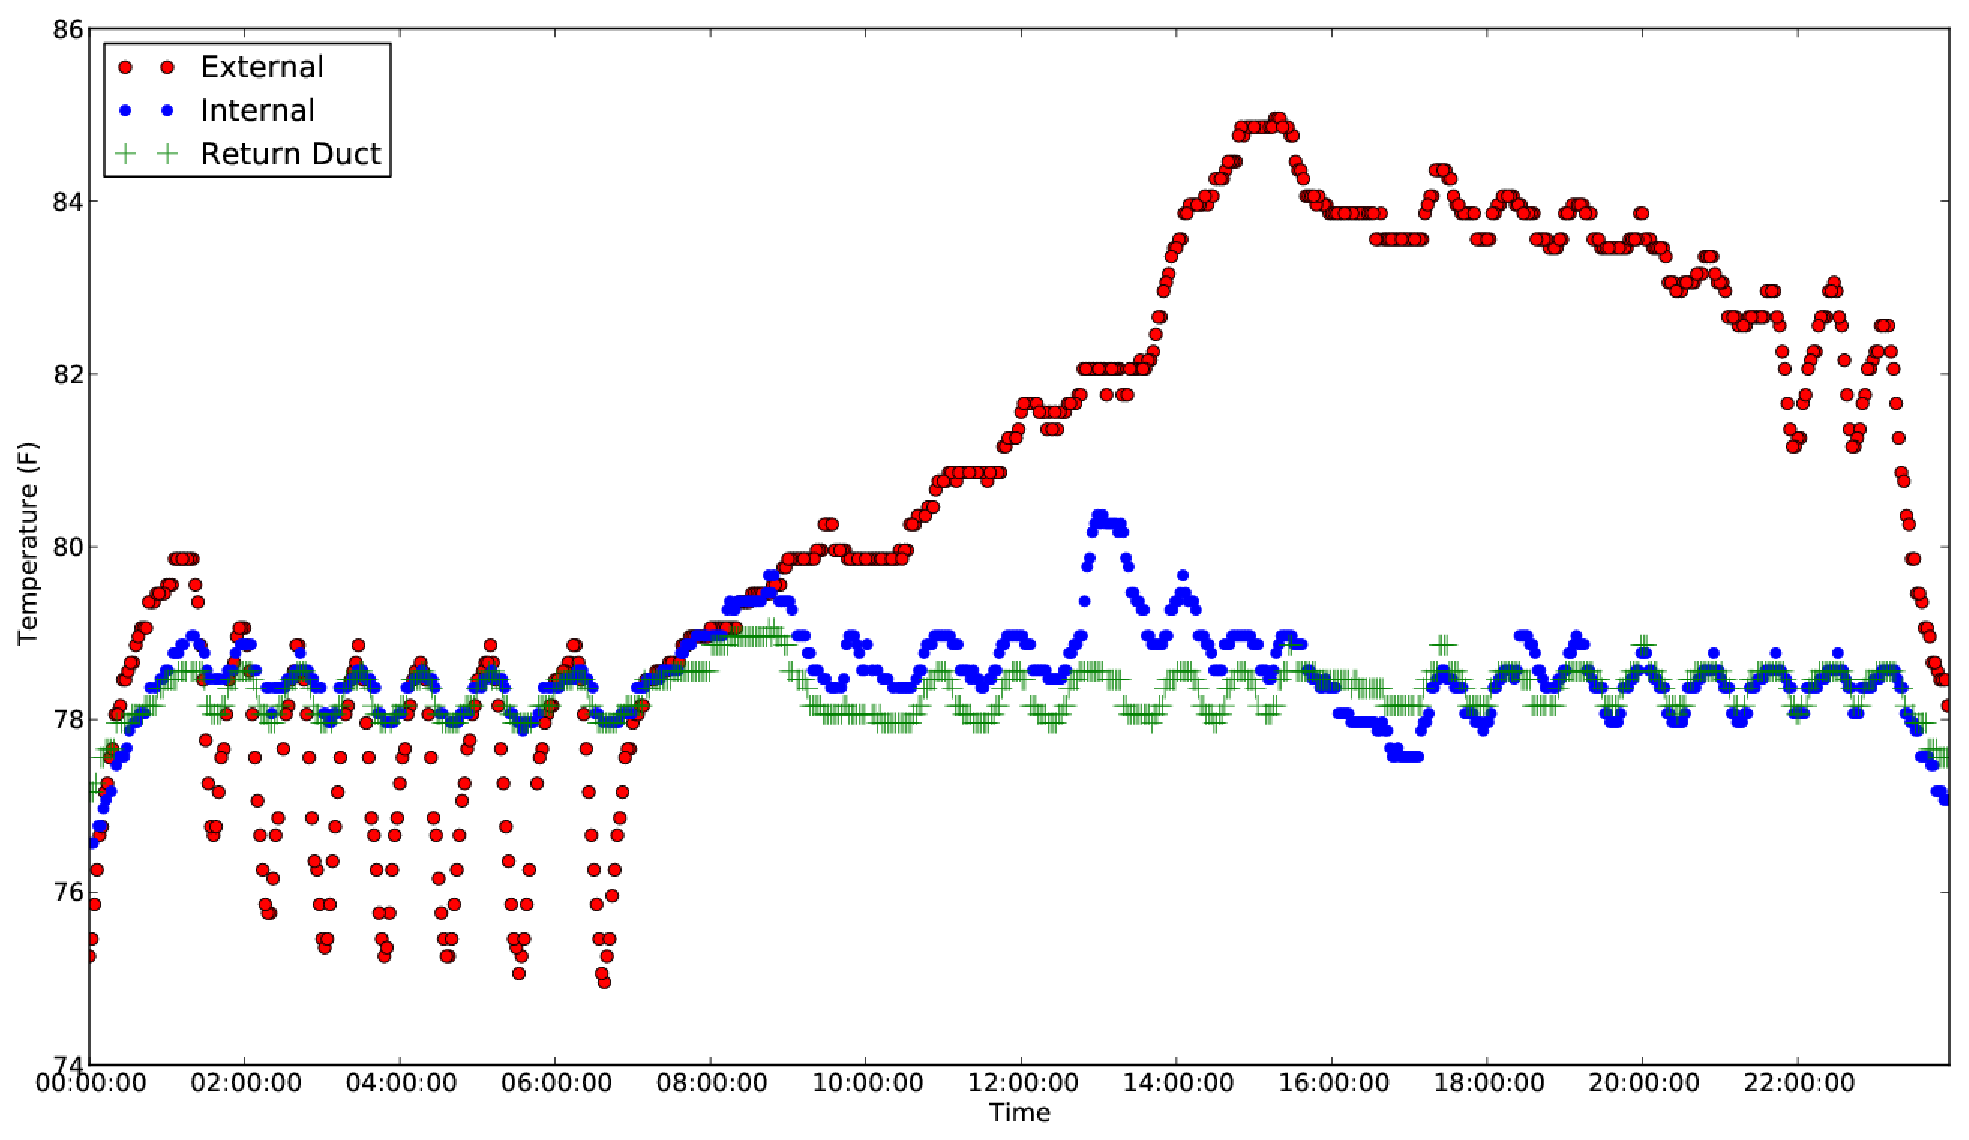
\includegraphics[width=0.6\columnwidth]{fig/intExtTherm.eps}
  \caption[Effect of Sensor Location on Temperature Reading]{The variation of
    temperature on a sensor placed on an internal wall, an external wall, and
    near the return duct.}
  \label{fig:intExtTherm}
\end{figure}

Figure~\ref{fig:intExtTherm} shows the temporal variations of several
temperature sensors placed throughout the house.  One sensor is placed
in the center of the house, directly in front of the only return
register, and therefore is exposed to a mix of air from all rooms.
Another sensor is placed on an internal wall of the house, and a third
sensor is placed on an external wall.  The figure shows that the
temperature sensor on the internal wall varies with the temperature of
the individual room, which is slightly more than the variation of the
centrally placed sensor.  However, the sensor on the external wall is
subject to wild temperature swings.  On the left side of the graph, it
is clear that the sensor has much greater downward swings than the
internal sensors.  This is because is it subject to direct air flow
from the ducts, which are typically placed on external walls.  It is
also subject to heat that concentrates around the window mid-day.
Because of these large temperature fluctuations, we decided to use
only sensors on the internal walls of each room: the temperature in a
zone was calculated as the average of the temperatures of each of the
internal sensors in the rooms comprising the zone.

\section{Controlling Air-flow into Rooms}
\label{sec:activeRegisters}

\begin{figure*}[t]
\centering{
\subfigure[1st Generation]{
\includegraphics[width=.4\columnwidth,height=.4\columnwidth,keepaspectratio=true]{./fig/RegisterGen1Front}
\label{fig:registerGen1}
}
\subfigure[2nd Generation]{
\includegraphics[width=.3\columnwidth,height=.3\columnwidth,keepaspectratio=true]{./fig/RegisterGen2Front}
\label{fig:registerGen2}
}
\subfigure[3rd Generation]{
\includegraphics[width=.3\columnwidth,height=.3\columnwidth,keepaspectratio=true]{./fig/RegisterGen3}
\label{fig:damper}
}
\subfigure[Bench-Top Test Rig]{
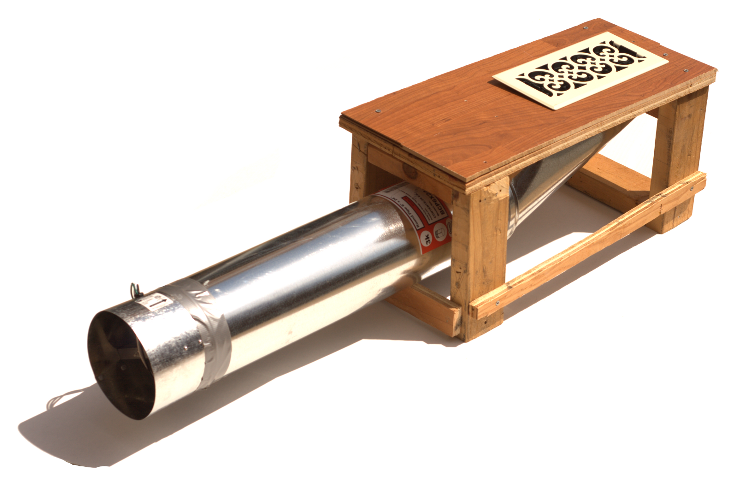
\includegraphics[width=.3\columnwidth,height=.3\columnwidth,keepaspectratio=true]{./fig/testRig}
\label{fig:testRig}
}
\caption[Three Generations of Active Registers and Bench-Top Test Rig]{Three
  generations of active registers.  (a) The first generation uses servo motors
  and a rotating louver design, but exhibited too much leakage.  (b) The second
  generation uses a sliding gate design to solve the leakage problems, but
  causes too much noise.  (c) The third generation uses an in-line duct
  damper. (d) The bench-top test rig used to verify that the second generation
  wirelessly controlled active registers have almost no air leakage.}
\label{fig:activeRegisters}
}
\end{figure*}

In order to control the airflow into individual rooms, we designed and built
{\em active registers and dampers} that can be wirelessly opened or
closed. While controllable registers are commercially available, they actuate
based on either preset temperatures or temporal schedules. Commercial active
registers that are controllable via a remote control would be hard to integrate
with our wireless control system and such registers are expensive, costing over
\$50 each. Our designs improved through three generations as shown in
Figure~\ref{fig:activeRegisters}. We implemented the registers using cheap,
off-the-shelf (COTS) components including an operable register, a servo motor,
and a small amount of custom circuitry. These components resulted in a cost of
less than \$20 per register excluding the cost of the TelosB mote, which was
used for wireless communication. Building on results of previous
studies~\cite{TRANE2003, walker2008residential, watts2007application}, we used
the experimental bench-top testing framework shown in Figure~\ref{fig:testRig}
to verify that the second generation active registers block nearly 100\% of
airflow. The third generation active dampers are used in professionally
implemented zoned HVAC systems and cost about \$50 each. Several prototypes and
even commercial versions of similar hardware are currently
available~\cite{walker2003register,walker2008residential,watts2007application}.
Our system goes beyond these devices by integrating them into a cooperative,
wireless system.

\begin{figure}[ht]
  \centering
  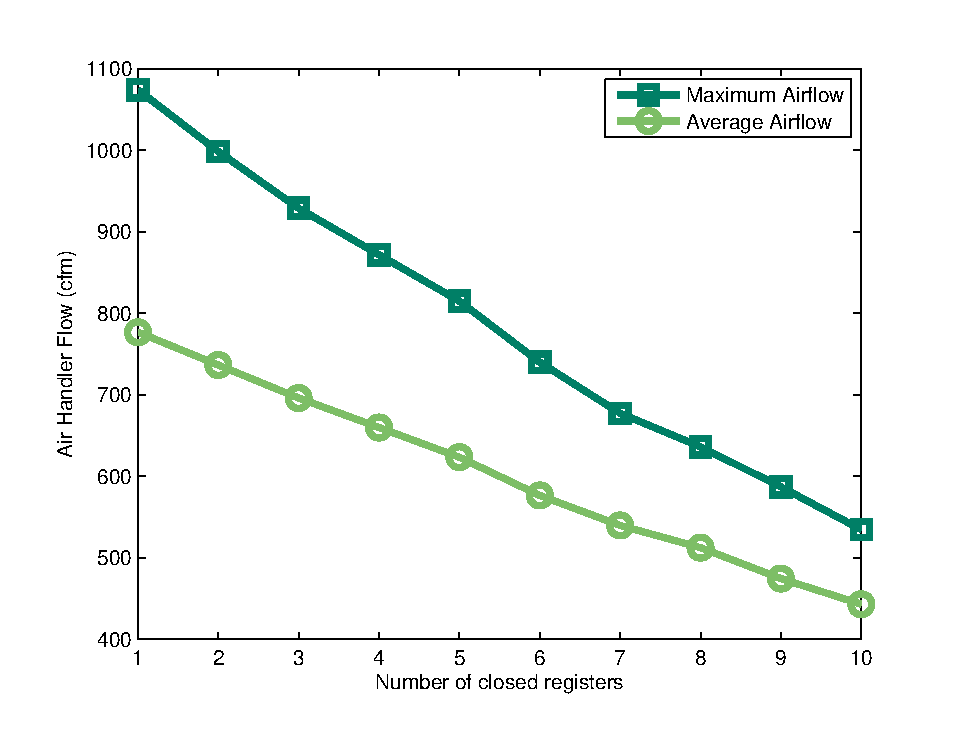
\includegraphics[width=0.6\columnwidth]{fig/regClosingAirflow.eps}
  \caption[Effect of Closing Registers on Air Flow]{As more registers are
    closed, some efficiency is lost and the total total air volume output by the
    system decreases.}
  \label{fig:regClosingAirflow}
\end{figure}

We measured the effectiveness of the second generation registers at directing
airflow into different rooms using a Kestrel 4100 Pocket Air Flow Tracker
manufactured by Nielsen-Kellerman~\cite{kestrel}. This sensor is placed above
the register and provides a measure of airflow in terms of cubic feet per minute
(CFM) that is coming out of the register.  This measurement is based on the
known size of the register and the speed of the air.
Figure~\ref{fig:regClosingAirflow} shows that the total airflow coming from all
registers is reduced as an increasing number of registers are closed.  When all
registers are open, the average airflow is approximately 800 CFM, which matches
the specification of the air handler in this house.  However, as more registers
are closed, the average airflow approaches 450 CFM, which is almost half. Total
airflow does not approach zero because some air escapes even from the closed
registers.  This result verifies that closing registers does decrease the
overall efficiency of the system because it reduces the total airflow output, as
suggested by~\cite{walker2003register}.  Therefore, actively cooling only half
the house would not cause double the amount of air to be available to the cooled
zone, because some air is lost due to backpressure, increased duct friction,
duct leakage, and leakage from the closed registers.


\section{Controlling the HVAC System}
\label{sec:controllingHVAC}
